\section{Problem Formulation}
\label{sec:formulation}

We model a single migration event, where a source site must move its active inference
sessions to other sites before a deadline $D$ so that the source can shed power.
For each session the decision is \emph{where} it lands and \emph{how} its serving
state is rebuilt there. We call the controller that plans and routes this migration
\emph{Queue-Haul} (Fig.~\ref{fig:sites}), since it queues sessions at the source and moves
their state to the destinations.

\begin{figure}[t]
\centering
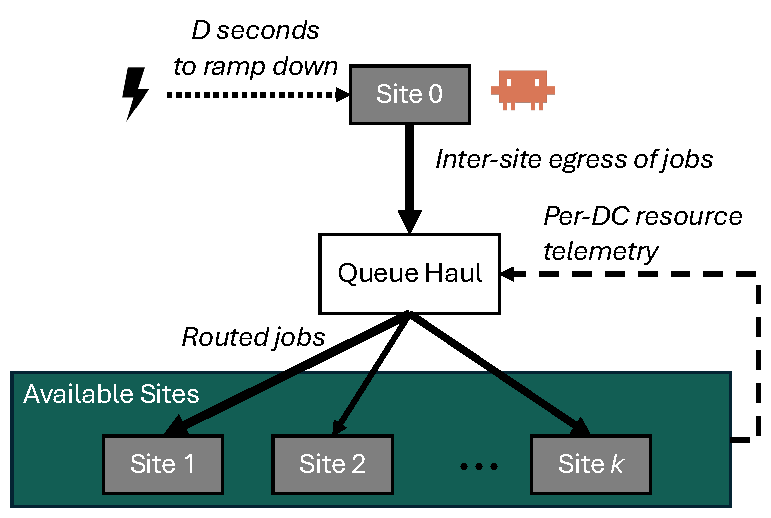
\includegraphics[width=0.8\linewidth]{queue-haul-sites.pdf}
\caption{Queue-Haul in context. A source site (Site~0) under a $D$-second ramp-down
egresses its stateful sessions to the controller, which routes them across
available destination sites using per-datacenter resource telemetry.}
\label{fig:sites}
\end{figure}

Sessions are grouped into classes $q\in\mathcal{Q}$ by model $m(q)$ and
token-length bucket, and class $q$ holds $n_q$ jobs of context length $T_q$. A job is
rebuilt at a destination $\ell\in\mathcal{L}$ by one of two actions.
\emph{Replay} ($R$) ships the compact context ($\beta_q T_q$ bytes, with
$\beta_q\!=\!4$\,B/tok) and recomputes the KV cache through prefill, costing
$T_q/\rho_q$ GPU-seconds on an instance already serving the model. \emph{State transfer} ($S$) ships the
KV cache itself ($\eta_q T_q$ bytes, $\eta_q$ the per-token KV size) and skips
prefill, paying instead to ingest that volume. The decision variables are the
fractional job counts $x^R_{q\ell},x^S_{q\ell}\ge 0$ and the \emph{stranded} count
$z_q\ge 0$ of jobs not rebuilt by the deadline. We relax $x,z$ to the reals, so the
program is a planning model for how much work moves, where, and by which action.
The relaxation models fractional jobs whose loads are integrated over the window
$[0,D]$. It does not model intra-window ordering or transient queueing.

\paragraph{Resource model.} Each destination has three resources shared over the
window $[0,D]$, namely network ingress $\Lambda_\ell$ and, per model, a GPU
pool $W_{\ell m}$ that serves both prefill and state ingest (the latter at
per-instance rate $\mu_{\ell m}$). Capacities scale with the deadline,
\[
C^{\mathrm{net}}_\ell=\Lambda_\ell D,\quad
C^{\mathrm{pfill}}_{\ell m}=W_{\ell m} D,\quad
C^{\mathrm{ing}}_{\ell m}=W_{\ell m}\mu_{\ell m} D,
\]
and the induced loads are affine in $x$,
\[
\begin{aligned}
L^{\mathrm{net}}_\ell &= \textstyle\sum_q\big(\beta_q T_q\,x^R_{q\ell}+\eta_q T_q\,x^S_{q\ell}\big),\\
L^{\mathrm{pfill}}_{\ell m} &= \textstyle\sum_{q\in\mathcal{Q}_m}\tfrac{T_q}{\rho_q}\,x^R_{q\ell},
\qquad
L^{\mathrm{ing}}_{\ell m} = \textstyle\sum_{q\in\mathcal{Q}_m}\eta_q T_q\,x^S_{q\ell}.
\end{aligned}
\]
Replay loads prefill but is light on the network for long contexts. State transfer
loads network and ingest but never prefill. We let $p_i(x)=L_i(x)/C_i$ be the
normalized pressure on resource $i$ in the index set $\mathcal{I}$. Every stage
shares the same base constraints,
\[
\sum_{\ell}\big(x^R_{q\ell}+x^S_{q\ell}\big)+z_q=n_q\ \ \forall q,
\qquad
p_i(x)\le 1\ \ \forall i\in\mathcal{I}.
\]
The equality conserves jobs, so each one either moves or is stranded, and the unit
ceiling holds every resource within its window budget.

The goals here pull in different directions and live in different units. We want to
migrate every class fairly, spread the load, keep the worst class's rebuild cheap,
and keep the classes even with one another. Folding them into one weighted objective
would bury whichever matters most, so we take them in strict priority order, or
\emph{lexicographically}. Each stage optimizes one objective, freezes its optimum
as a constraint, and hands the problem down. The four stages are the four boxes of
Fig.~\ref{fig:pipeline}.

\smallskip\noindent\textbf{Stage 1, proportional-fair allocator (convex).} After trying many objectives, we kept hitting a \emph{fairness} problem, where the smaller jobs always move first. To spread which jobs get moved more evenly, we use a proportional-fair allocator. We score each class by the log of the
fraction it gets to move, weighted by its size, and maximize the total,
\[
\max_{x,z\ge 0}\ U(z)=\sum_q n_q\log\!\Big(1-\tfrac{z_q}{n_q}\Big)
\quad\text{s.t. base constraints.}
\]
The migrated fraction of class $q$ is $1-z_q/n_q$, so stranding a class outright
sends its term to $-\infty$. The optimum therefore never starves one class to help
the total. When the deadline is generous everyone moves ($z=0$, $U^\star=0$), and
when it is tight the unavoidable shortfall spreads across classes rather than
concentrating on a few. The optimal value $U^\star$ is a fairness guarantee, and every
later stage carries $U(z)\ge U^\star-\delta$ for a small $\delta$, so the fair
allocation survives to the final plan. (Swapping $U$ for $\sum_q z_q$ or a max--min
floor recovers job-count throughput or other variants.)

\smallskip\noindent\textbf{Stage 2, minimize peak resource pressure (LP).} The fair
allocation can still lead to imbalances in the replay or state-transfer mix, so the next step is to minimize the peak pressure $\phi$ over all resources, which is a min--max LP,
\[
\min_{x,z,\phi}\ \phi \quad\text{s.t. }
p_i(x)\le\phi\ \forall i,\ \ U(z)\ge U^\star-\delta,\ \text{base constraints.}
\]
$\phi^\star$ is the lowest achievable peak utilization. Below $1$ the plan has
slack, and at $1$ some resource is saturated. This is the workhorse stage, where
the replay-versus-transfer split and the choice of destination are settled, and its dual prices
(Sec.~\ref{sec:methods}) are the shadow prices we later put to use. Many plans hit the
same peak, so we use a tie-breaking QP
$\min\tfrac12\sum_i p_i(x)^2$.

\smallskip\noindent\textbf{Stage 3, minimize the worst-class cost (LP).} The last
two stages judge a plan by each class's rebuild cost,
\[
r_q=\tfrac{1}{n_q}\big[\textstyle\sum_\ell(c^R_{q\ell}x^R_{q\ell}+c^S_{q\ell}x^S_{q\ell})+d^{\mathrm{miss}}z_q\big],
\]
with $c^a_{q\ell}$ the unloaded reconstruction time and $d^{\mathrm{miss}}\!=\!2D$
the stranded-job penalty. Stage 3 caps the worst class, $H=\max_q r_q$.

\smallskip\noindent\textbf{Stage 4, minimize spread between classes (LP).}
Finally, we even the classes out by minimizing the spread $V=\max_q|r_q-\bar r|$, so no
class sits far from the average. Each stage freezes the previous optimum, so the
fair allocation and the balanced load both carry through to the end.

\paragraph{Convexity.} Every stage is convex over the same polyhedron (affine
conservation and capacity constraints, nonnegativity). Stage 1 maximizes a concave
sum of logs (an exponential-cone program), Stage 2 is a min--max LP with a QP
tie-break, and Stages 3 and 4 are LPs, so the pipeline runs
conic\,$\to$\,LP\,$\to$\,LP\,$\to$\,LP. Every local optimum is global and strong
duality holds, which is exactly what makes the Stage-2 prices in the next section
meaningful.
